% Style files vendored from https://github.com/JmlrOrg/tmlr-style-file
% commit 7bf90efe3a0debbba703c05c43f3ff7e4d4a2992 (Apache-2.0; see TMLR_STYLE_LICENSE.txt).
% Draft dated 10-18-2026. Default tmlr options hide authors, matching a TMLR submission.
% Camera-ready would switch to \usepackage[accepted]{tmlr}. This PDF is not a submission.
\documentclass[10pt]{article}

\usepackage{tmlr}
\usepackage{hyperref}
\usepackage{url}
\usepackage{graphicx}
\usepackage{booktabs}
\usepackage{amsmath}
\usepackage{xcolor}
\usepackage{array}

\providecommand{\todocite}[1]{\textcolor{red}{[CITE: #1]}}

\title{Training History Reverses Observed Difficulty\\on a Fixed Addition Task}

% Authors are hidden unless tmlr is loaded with the accepted or preprint option.
% Affiliation and coauthors are unresolved. Do not treat this block as a submission list.
\author{\name Brando Miranda \email brando9@stanford.edu \\
      \addr Affiliation and coauthors not yet confirmed}

\def\month{10}
\def\year{2026}
\def\openreview{\url{https://openreview.net/forum?id=XXXX}}

\begin{document}

\maketitle

% !TEX root = main.tex
\begin{abstract}
% CS197 move 1: problem motivation (failure mode) -- a score confounds task demand with practice.
A measured score confounds what a task demands with what a learner has practiced.
% CS197 move 2: assumption (setup bit) -- the ranking is treated as a property of the item.
Accounts of difficulty often treat the resulting ranking as a property of the item.
% CS197 move 3: contribution (bit flip) -- changing the training mixture reverses the ranking.
On exact addition of two three-digit integers, changing only the training mixture reverses which items look harder.
% CS197 move 4a: instantiation (fixed skill) -- items, checker, and algorithm stay fixed.
The test items, the exact-sum checker, and the addition algorithm stay fixed.
% CS197 move 4b: instantiation (learners and probe) -- small networks plus a starting-loss probe.
The learners are small two-hidden-layer networks, and an independent starting-loss probe forecasts later loss.
% CS197 move 5a: evaluation (ranking) -- answer-matched reversal, eight seeds, fixed items. Source: experiments/archive/03_answer_matched_alignment/RESULTS_matched_alignment.md.
Answer-matched training gives a 25.30-point no-carry lead [23.14, 27.26] and a 24.58-point two-carry lead [22.88, 26.19].
% CS197 move 5b: evaluation (probe needs heterogeneous history) -- 05 and 07 supported; 04 below the 10% line. Sources: RESULTS_history_retention.md, RESULTS_mdl_history.md, RESULTS_stable.md.
That probe cuts joint held-out loss error by 47.20\% [42.88, 53.08] after heterogeneous pretraining, and by 36.22\% [32.45, 40.51] when carry rates are also matched.
Under one shared warmup the same probe adds 3.48\% [1.12, 6.24], below a prespecified 10\% line.
% CS197 move 5c: evaluation (failed gates, equal prominence) -- 01 retention, 07 accuracy line, 08 utility law.
Online code length and verifiable-reward gains reverse with history as well.
Frozen gates still fail: the first study drops control accuracy by 6.08 points, a later two-carry pool reaches 81.09\% [79.51, 82.88] against an 85\% line, and an additive utility law changes pooled error by $-15.78\%$ [$-35.91$, $3.15$].
% CS197 move 5d: evaluation (headroom repair supported; probe inside the bound not established) -- experiments/archive/09_headroom_bounded_rlvr_utility_law/RESULTS_headroom_bounded.md and expt_v1/results/gates.json. Relative reductions 0.7372120580111765 [0.7042625604099736, 0.7725511008836561] and 0.08097966173425564 [0.02517020100878975, 0.1438982595691034]. Stored intervals, not redrawn. p-val=n/a.
The headroom bound in \texttt{experiments/archive/09\_headroom\_bounded\_rlvr\_utility\_law/} is supported, with a 73.72\% [70.43, 77.26] relative reduction in joint root mean squared error, but probe features inside that bound are not established, at 8.10\% [2.52, 14.39].
% CS197 move 6: implication (scope) -- this task and these networks, not language models.
The measurements cover this addition task and these networks.
They do not show that difficulty is mostly data for language models or public benchmarks.
\end{abstract}

% !TEX root = main.tex
\section{Introduction}
% paragraph 1: problem motivation. Same claim as abstract sentence 1.
Observed difficulty moves when training exposure moves, even if the scored skill stays fixed.
A reported score then mixes the task with the learner's preparation.
That mix matters when a low score is later read as a property of the task.
We keep one skill fixed and change the training mixture on purpose.
The skill is exact addition of two zero-padded three-digit integers, scored by exact equality of the sum.
The addition algorithm and the test items stay fixed inside each comparison.
The open question is how much of the measured ranking is exposure.

% paragraph 2: prior assumption. Rankings are stated without the training history under test.
A common assumption is that item structure fixes the ranking before any training history is named.
Conditional description length, for a fixed machine, input, answer, and task, is one such structural quantity \citep{kolmogorov1968three,grunwald2008algorithmic}.
It does not change across our exposure conditions, because those arguments do not change.
Resource laws instead predict average loss from parameter count and data or compute \citep{kaplan2020scaling,hoffmann2022chinchilla}.
They still do not name which items a particular network has practiced.
Curriculum methods order examples by a chosen difficulty signal \citep{bengio2009curriculum}.
Compositional benchmarks show that success depends on how primitives are recombined between training and test \citep{lake2018generalization,keysers2020measuring}.
The shared gap is a ranking stated without the history being tested.

% paragraph 3: contribution. The ranking follows the mixture; the probe helps only when histories differ.
In these experiments the ranking follows the training mixture.
The same items look hard under one mixture and easy under another, at a matched budget.
A starting-loss probe, measured on held-out items before the later training stage, records how much of that history the network absorbed.
The probe improves held-out forecasts when starting checkpoints have different histories.
It adds little when every checkpoint shares one warmup.
The probe is a measurement of a trained network, not an intrinsic label of an item.

% paragraph 4: instantiation. Nine prespecified studies, monotone ridge, online code length, verifiable reward, headroom bound.
We report nine studies that were frozen before their outcomes.
The networks have two hidden rectified layers, six one-hot input digits, and four digit heads.
Early studies vary carry exposure with a shared architecture and budget.
Later studies match answer histograms, and then also match per-column carry rates.
Forecasts use a constrained monotone ridge on log loss, fit on calibration outcomes and scored on held-out widths and mixtures.
One study scores an online description length along the adaptation stream \citep{rissanen1978modeling,voita2020information}.
One study replaces supervised updates with a 0/1 exact-sum reward and a leave-one-out group-relative update \citep{shao2024deepseekmath}.
\texttt{experiments/archive/09\_headroom\_bounded\_rlvr\_utility\_law/} keeps that reward and caps the utility forecast by remaining headroom.
Table~\ref{tab:gates} states every prespecified decision, including the ones that fail.

% paragraph 5: evaluation. Supported results and failed gates, one claim per sentence.
Answer-matched exposure reverses the no-carry versus two-carry ranking at every tested width.
The two endpoint leads are 25.30 [23.14, 27.26] and 24.58 [22.88, 26.19] percentage points.
After heterogeneous pretraining, adding the starting-loss probe cuts joint held-out root mean squared error by 47.20\% [42.88, 53.08].
With per-column carry rates matched, the same comparison cuts loss error by 36.22\% [32.45, 40.51] and online description-length error by 56.93\% [55.01, 58.67].
A verifiable-reward stage cuts post-training loss error by 39.87\% [36.20, 50.17], and the accuracy gain itself reverses with history.
The failures are part of the same record.
The first balanced-exposure study recovers most of a long-carry gap and still misses its retention gate, because no-carry accuracy falls by 6.08 points.
A later remediation pool recovers its gap and still misses an 85\% accuracy line, at 81.09\% [79.51, 82.88].
An additive utility law worsens pooled held-out error by 15.78\%, with interval [$-35.91$, $3.15$].
The headroom bound in that study is supported, with relative root mean squared error reduction 73.72\% [70.43, 77.26].
Probe features inside the bound are not established, at 8.10\% [2.52, 14.39].
Every interval above is a percentile interval over eight seed blocks, and the decision rule uses the interval rather than a separate test (p-val=n/a), except for one auxiliary sign-flip test named in Section~\ref{sec:ranking}.

% paragraph 6: implications and contributions.
A difficulty report for this task should name the learner, the training history, and the budget.
We do not estimate what share of public-benchmark difficulty is data.
We do not claim that these networks implement one shared internal algorithm.
\begin{itemize}
\item Exposure reverses observed addition difficulty on fixed items, including after answer matching and after per-column carry matching.
\item A starting-loss probe improves held-out loss forecasts when pretraining histories differ, and it stays below a 10\% line when they do not.
\item The reversal also appears in online description length and in verifiable-reward improvement, beside prespecified gates that fail.
\item A headroom bound repairs the failed additive utility law on fresh seeds.
\item Probe features inside that bound stay below the prespecified 10\% line.
\end{itemize}

% !TEX root = main.tex
\section{Related work}
% Each prior-work sentence carries its own gap. No claim that this paper studies language models.

\paragraph{Description length.}
\citet{kolmogorov1968three} measure information by the shortest program that produces an object on a fixed machine.
\citet{grunwald2008algorithmic} separate that description length from the time the program takes to run.
\citet{rissanen1978modeling} selects models by total description length, charging for the model as well as the data.
Final cross-entropy under a trained network omits that charge.
\citet{voita2020information} make the charge operational by coding labels online, before each update of a fixed learning rule.
Our online code in \texttt{experiments/archive/07\_prequential\_mdl\_and\_length\_transfer/} follows that prequential pattern on the addition stream.
It is not an estimate of Kolmogorov complexity.
The conditional complexity of each test pair stays fixed because the input, the answer, the task statement, and the reference machine stay fixed.

\paragraph{What a ranking is attached to.}
\citet{bengio2009curriculum} train on easier examples before harder ones, using a difficulty signal chosen in advance.
That design is useful when the order is stable.
Our measurements ask whether the order stays put after the mixture changes.
\citet{lake2018generalization} find that sequence models can fit a compositional training set and still miss systematic recombinations.
\citet{keysers2020measuring} separate a match of primitive distributions from a match of their compositions.
Those papers study sequence tasks.
Our carry design is a smaller arithmetic version of the same question, with an exact checker and a frozen test set.
\citet{zhang2017understanding} show that deep networks can fit random labels of a finite training set.
Fitting those labels does not predict independent random labels on new items.
Our shuffled-label control is the addition analogue: exact-sum accuracy stays near zero.

\paragraph{Resource laws and metric artifacts.}
\citet{kaplan2020scaling} and \citet{hoffmann2022chinchilla} predict language-model loss from scale and from data or training compute.
Those laws describe average loss.
They do not identify which evaluated items were in the training mixture.
We borrow only the idea of a simple law in parameter count and updates, then test extra covariates on addition networks.
This is not a scaling-law result for language models.
\citet{power2022grokking} show that, on small algorithmic tasks, generalization can arrive long after the training loss has fallen.
Their intervention is training time under one data distribution.
Ours holds the scored budget fixed inside a comparison and changes the mixture.
\citet{schaeffer2023mirage} show that an aggregate metric can create an apparent jump in capability.
That paper is about metric discontinuities on language-model benchmarks.
This paper is about training history on one addition task.
We cite it only as a neighboring warning against reading a score as a property of the task.

\paragraph{Group-relative updates.}
\citet{shao2024deepseekmath} introduce group relative policy optimization for language-model mathematics.
We use the name only for the leave-one-out advantage in our protocol, with group size 16 and a 0/1 exact-sum reward.
We do not train a language model, and we do not reproduce that paper's experiments.
The phrase in our last study means the reward is the exact-sum check.
A cleared public source for that phrase is still missing \todocite{public source for the name reinforcement learning with verifiable rewards}.
A cleared citation for a companion mathematics grid used in the second study is also unresolved.
That grid is described from the project report, not cited as a peer-reviewed law.

% !TEX root = main.tex
\section{Task, models, and decision rules}
\label{sec:setup}

\paragraph{Task.}
Every study scores exact addition of two integers from 000 to 999.
Inputs are six one-hot decimal digits.
The target is four output digits, including a possible thousands digit.
Accuracy requires all four digits to match the integer sum.
The loss we forecast is the sum of $-\log_2$ probabilities of the correct digits under a factorized head.
That quantity is a conditional code length in bits per answer, given the trained network.
It omits the cost of transmitting the network and the training data, except in the online code of Section~\ref{sec:mdl}.
An independent column-addition checker agrees with integer addition on all 500{,}500 unordered pairs before training.
Swapped operand pairs never cross a split.

\paragraph{Networks and optimization.}
The networks have two hidden rectified layers.
Widths 32, 64, 96, 128, and 384 have 4{,}328, 10{,}664, 19{,}048, 29{,}480, and 186{,}664 parameters in the later studies.
\texttt{experiments/archive/02\_heldout\_exposure\_difficulty\_laws/} and \texttt{experiments/archive/03\_answer\_matched\_alignment/} use width 256 (91{,}688 parameters) in place of width 384.
Optimization is AdamW with learning rate $10^{-3}$, weight decay $10^{-4}$, and 256 examples per update, except where a protocol states a different budget.
Seeds are the resampling unit.
Eight seeds are paired across mixtures inside a study.
Initialization and batch order are paired within a seed.
No seed or cell was dropped.

\paragraph{What is held fixed.}
Inside a comparison, the test-item identities, the checker, the optimizer, and the scored update counts stay fixed.
The training distribution changes.
Early studies change the fraction of long carry chains and also change digit and answer frequencies.
That identifies a distribution intervention, not a uniquely isolated effect of carrying.
Later studies remove those mismatches in stages.
Answer matching uses the same 117 sums, with the same count of training pairs per sum, in both strata.
Carry-rate matching further forces every mixture to have a 50\% ones-column carry rate and a 50\% tens-column carry rate.
Input-digit total variation is reported with those controls.
Total variation is half the sum of absolute differences over the ten digits.

\paragraph{Laws.}
A forecast law is fit inside each seed on calibration outcomes only.
Coefficients and forecasts are frozen before the analysis reads the final-test outcomes.
The joint holdout uses widths and mixtures that never enter the fit.
The primary score is root mean squared error (RMSE) on mean bits per answer, or on accuracy gain where the protocol says so.
Relative reduction is $100 \times (1 - \mathrm{RMSE}_{\mathrm{extended}} / \mathrm{RMSE}_{\mathrm{baseline}})$.
Positive means the extended law has lower error.
Mean bias is the forecast minus the observation.
A positive bias overpredicts loss or utility.
The unconstrained difficulty law that fails in Section~\ref{sec:forecasts} has the form
\begin{equation}
\label{eq:legacy}
\widehat{\mathrm{loss}}
= e^{a}\, N^{b}\, T^{c}\, e^{d \cdot s}\, q^{e}\, D^{f},
\end{equation}
with parameter count $N$, updates $T$, carry indicator $s$, exposure $q$, and starting loss $D$.
The stable laws replace unconstrained least squares with a ridge penalty of $0.01$ on standardized slopes.
Size, update, and exposure slopes are constrained to be nonpositive, and the starting-difficulty exponent is constrained to $[0,1]$.
Those bounds were frozen before the repair studies collected their trajectories.
A repair success does not substitute for a feature-value success.
The two gates are separate.

\paragraph{Uncertainty and thresholds.}
Intervals are 95\% percentile intervals from 20{,}000 paired bootstrap draws of eight complete seed blocks, unless a study states a different design.
Items inside a test set are not resampled as independent trials.
The intervals condition on the fixed items, architecture family, and holdout.
They do not cover other tasks or optimizers.
Where the protocol decides by the interval and a practical threshold, we report p-val=n/a.
The practical thresholds are project choices frozen in the protocols: usually a 10\% relative RMSE reduction, or a 10 percentage-point accuracy lead, together with a positive lower endpoint and a required pattern across widths.
They are not literature standards.
Table~\ref{tab:gates} lists the decision for every frozen gate we rely on.
Per-width means that were not given a fresh bootstrap are labeled as eight-seed means.

\begin{table}[t]
\centering
\small
\caption{\textbf{Prespecified gates both pass and fail.} Each row is one frozen decision from the named study under \texttt{experiments/archive/}.
Estimates use the published rounding in that study's results file.
Intervals are eight-seed block bootstraps with p-val=n/a.
A supported ranking does not imply that every width has a 10-point gap.
Full folder names and sources are in Appendix~\ref{app:gates}.}
\label{tab:gates}
\begin{tabular}{@{}p{0.20\textwidth}p{0.32\textwidth}p{0.27\textwidth}p{0.10\textwidth}@{}}
\toprule
Study & Decision & Estimate & Status \\
\midrule
01 fixed-width exposure & Gap recovery with retention & 94.34\% recovered; control $-6.08$ points & Not established \\
02 held-out laws & Exposure plus starting loss & 6.80\% [$-3.52$, $14.80$] & Not established \\
03 answer-matched & Ranking reversal & 25.30 and 24.58 points & Supported \\
03 answer-matched & Starting-loss forecast & $0.4727 \to 292.7941$ bits & Not established \\
04 monotone ridge & Repair versus unconstrained law & 100.00\% [$99.90$, $100.00$] & Supported \\
04 monotone ridge & Probe versus constrained base & 3.48\% [$1.12$, $6.24$] & Not established \\
05 history and retention & Probe versus constrained base & 47.20\% [$42.88$, $53.08$] & Supported \\
05 history and retention & No-harm remediation & control $+1.09$ [$+0.33$, $+1.89$] & Supported \\
05 history and retention & Repair versus legacy difficulty & $-0.82\%$ [$-1.11$, $-0.57$] & Not established \\
06 carry marginals & Compositional reversal & 22.35 and 17.74 points & Supported \\
06 carry marginals & Probe under a shared warmup & 1.94\% [$-3.10$, $6.50$] & Not established \\
07 online code length & Loss law and online-code law & 36.22\% and 56.93\% & Supported \\
07 online code length & Remediation accuracy line & 81.09\% [$79.51$, $82.88$] & Not established \\
08 verifiable reward & Post-training loss law & 39.87\% [$36.20$, $50.17$] & Supported \\
08 verifiable reward & Additive utility law & $-15.78\%$ [$-35.91$, $3.15$] & Not established \\
09 headroom bound & Headroom-bounded repair & 73.72\% [70.43, 77.26] & Supported \\
09 headroom bound & Probe features inside the bound & 8.10\% [2.52, 14.39] & Not established \\
\bottomrule
\end{tabular}
\end{table}

% !TEX root = main.tex
\section{Exposure reverses the ranking}
\label{sec:ranking}

\subsection{A large exposure effect that misses retention}
\label{sec:exp01}
% Provenance: experiments/archive/01_fixed_width_addition_exposure/RESULTS_addition_exposure.md
In \texttt{experiments/archive/01\_fixed\_width\_addition\_exposure/}, one 29{,}480-parameter network is trained from scratch for 3{,}000 updates on 16{,}000 pairs.
The fixed test set has 1{,}000 pairs in each carry-chain length, evaluated under eight seeds (8{,}000 predictions per cell, not 8{,}000 independent items).
With 97\% no-carry training, no-carry accuracy is 100.00\% [100.00, 100.00] and length-three-carry accuracy is 9.60\% [7.85, 11.22].
With 97\% length-three-carry training, those same groups score 6.84\% [5.79, 7.79] and 100.00\% [100.00, 100.00].
Balanced training moves length-three accuracy from 9.60\% to 94.89\% (7{,}591/8{,}000) and recovers 94.34\% [92.74, 95.86] of the 90.40-point baseline gap.
The prospective retention rule allows no-carry accuracy to fall by at most 5 points.
It falls from 100.00\% to 93.92\%, a change of $-6.08$ [$-8.39$, $-4.11$] percentage points.
Five of six frozen criteria pass, and the aggregate verdict is not established.
An auxiliary sign-flip test of the length-three gain against half the baseline gap gives p-val=$0.00390625$ under an exhaustive paired sign enumeration.
That test does not override the failed retention criterion.
The shuffled-label control scores 22/32{,}000 exact sums (0.06875\%), below the protocol's 5\% ceiling.
Balanced training also makes length-one chains less accurate than length-three chains (73.92\% versus 94.89\%).
Carry-chain length is therefore not an empirically monotone difficulty scale in this run.
The extreme mixtures also change digit and answer frequencies, so the contrast is the whole distribution intervention.

\subsection{Answer matching preserves the reversal}
\label{sec:exp03}
% Provenance: experiments/archive/03_answer_matched_alignment/RESULTS_matched_alignment.md
\texttt{experiments/archive/03\_answer\_matched\_alignment/} gives every intervention exactly 40 training pairs for each of 117 sums (4{,}680 pairs).
The two evaluation strata have identical answer histograms, with 936 fixed items each.
After 500 shared balanced warmup updates, a 90\% no-carry intervention favors no-carry items by 25.30 [23.14, 27.26] percentage points at 3{,}000 updates.
A 90\% two-carry intervention favors two-carry items by 24.58 [22.88, 26.19] points.
Seed standard deviations of those two contrasts are 3.21 and 2.56 points.
Both lower endpoints are positive, and both contrasts are positive at each of the five widths.
The frozen ranking gate is supported.
The lead shrinks with width: 66.16 and 67.49 points at width 32, and 2.30 and 1.46 points at width 256.
The gate requires a pooled lead of at least 10 points and a positive point at every width.
It does not require a 10-point lead at every width.
Figure~\ref{fig:alignment} shows the reversal.
Input-digit total variation between the endpoint mixtures remains large, from 0.0668 to 0.6469 across the six digit positions.
Answer matching does not isolate carrying from the input digits.

\begin{figure}[t]
\centering
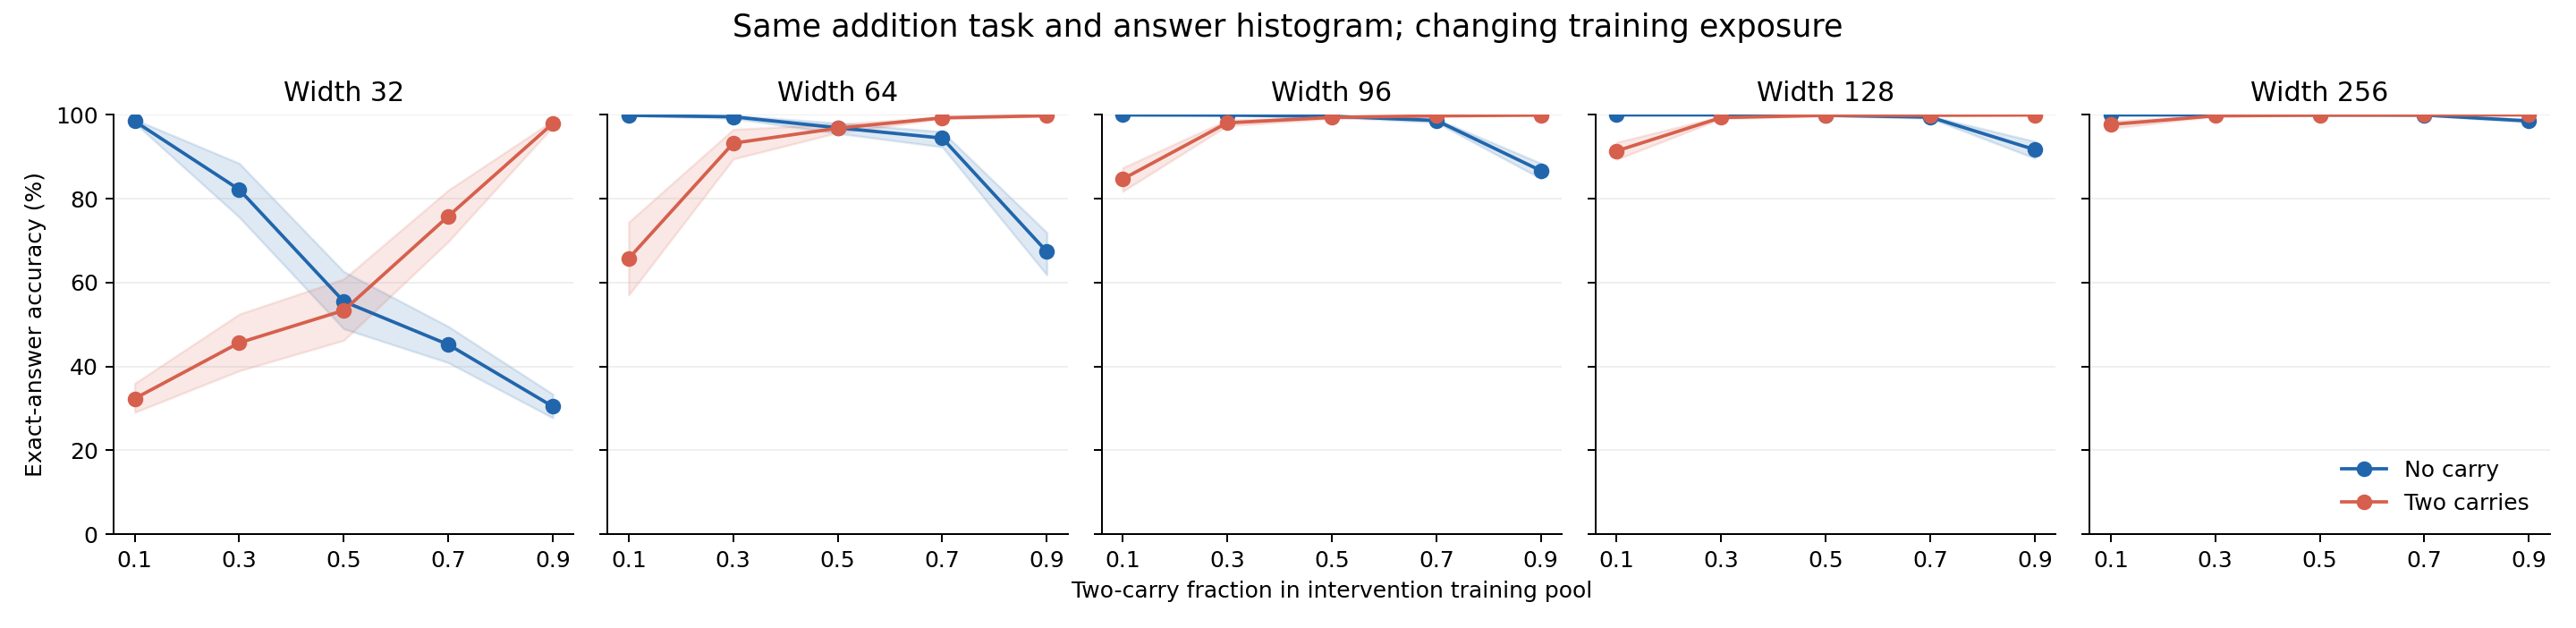
\includegraphics[width=\linewidth]{../../experiments/archive/03_answer_matched_alignment/expt_v1/results/alignment_accuracy.png}
\caption{\textbf{Answer-matched exposure reverses which stratum is more accurate.} Accuracy of no-carry and two-carry items against the two-carry training fraction, for \texttt{experiments/archive/03\_answer\_matched\_alignment/}.
Shading in the source figure is the paired-seed interval.
Eight seeds, 936 fixed items per stratum, p-val=n/a.
The same items change rank as the mixture changes.}
\label{fig:alignment}
\end{figure}

\subsection{The reversal survives matched carry rates}
\label{sec:exp06}
% Provenance: experiments/archive/06_compositional_carry_marginal_matched/RESULTS_compositional.md
% and expt_v1/results/prediction_comparisons.csv for the repair row.
\texttt{experiments/archive/04\_monotone\_ridge\_heldout\_addition/} repeats the answer-matched reversal on fresh items, seeds, and widths.
The endpoint leads are 24.07 [22.80, 25.46] and 24.48 [22.77, 26.06] percentage points, and the ranking gate is supported.
At width 384 the leads are 0.55 and 0.24 points, still positive and far below the pooled 10-point bar.
\texttt{experiments/archive/06\_compositional\_carry\_marginal\_matched/} then matches both the answer histogram and the per-column carry rates.
Every mixture has exactly 3{,}600/7{,}200 ones-column carries and 3{,}600/7{,}200 tens-column carries.
Endpoint input-digit total variation falls from a mean of 0.443 (maximum 0.656) in the previous answer-matched studies to a mean of 0.0398 (range 0.0049 to 0.0972).
The contrast is between isolated single carries, ones-only or tens-only, and a cascading two-carry cell.
At a 10\% compositional mixture, single carries lead by 22.35 [20.60, 24.00] points.
The two single-carry cells score 93.62\% [91.51, 95.60] and 93.78\% [91.93, 95.55], against 71.35\% [69.31, 73.66] on the two-carry cell.
At a 90\% compositional mixture, the two-carry cell leads by 17.74 [14.62, 21.12] points.
That cell scores 92.13\% [90.07, 94.07], against 74.28\% [70.55, 77.38] and 74.49\% [71.23, 77.84] on the single-carry cells.
Both directions are positive at all five widths, and the ranking gate is supported.
The residual structure contrast is 2.30 [1.02, 3.51] points, much smaller than the 20.05 [17.75, 22.32] alignment contrast.
Matching the column rates does not remove the reversal.
It also does not make the reversal the same size at every width: width 384 leads by 7.04 and 3.01 points.

% !TEX root = main.tex
\section{When starting loss improves a forecast}
\label{sec:forecasts}

\subsection{Shared warmups}
% Provenance: experiments/archive/02_heldout_exposure_difficulty_laws/RESULTS_heldout_laws.md
% experiments/archive/03_answer_matched_alignment/RESULTS_matched_alignment.md
% experiments/archive/04_monotone_ridge_heldout_addition/RESULTS_stable.md
% experiments/archive/06_compositional_carry_marginal_matched/results.md
% experiments/archive/06_compositional_carry_marginal_matched/expt_v1/results/prediction_comparisons.csv
\texttt{experiments/archive/02\_heldout\_exposure\_difficulty\_laws/} fits an additive resource law on widths 32, 64, and 128 and on three training fractions, then scores widths 96 and 256 and two held-out fractions.
There are 384 joint targets, 48 per seed.
Adding log exposure and probed starting loss reduces joint RMSE by 6.80\% [$-3.52$, $14.80$], from 1.2969 [1.2015, 1.3780] to 1.2087 [1.0941, 1.3590] bits per answer.
The primary gate required 10\%, a positive lower endpoint, and improvement at both held-out widths.
It is not established.
The difficulty-only ablation, which was secondary, reduces error by 15.80\% [10.27, 20.52].
Adding log exposure on top of that ablation worsens held-out error by 10.69\% (relative reduction $-10.69\%$ [$-20.54$, $-2.54$]).
The difficulty-only law produces 52/384 negative loss forecasts, and the combined law produces 64/384.
Mean bias for the combined law is $-0.1597$ bits (forecast 2.9539, outcome 3.1135).
A companion grid of 24 mathematics observations, four model sizes at a fixed token budget, tests a training-breadth proxy rather than measured exposure or starting loss.
Adding the proxy changes joint error by $-1.14\%$ [$-9.58$, $0.57$], a descriptive interval over four size blocks.
That companion does not validate the addition result on language models, and the addition result does not replace it.

\texttt{experiments/archive/03\_answer\_matched\_alignment/} changes the functional form to Equation~\eqref{eq:legacy} and the forecast fails.
Joint RMSE rises from 0.4727 [0.3212, 0.5990] to 292.7941 [0.3588, 507.0797] bits per answer, a relative reduction of $-61835.64\%$ [$-140226.76$, $27.71$].
The feature-value gate is not established.
One seed, whose starting-loss exponent is $-7.1966$, contributes 99.9677\% of the joint squared error.
Its worst forecast is 2737.3272 bits against an observed 0.0932.
The fit saw starting losses only from 2.5316 to 3.9151 bits, while a held-out network reached 0.5135.
A negative exponent treats a better starting point as a reason to predict a worse outcome once the probe leaves the fitting range.
This diagnosis was written after the failure.
It does not drop the seed or change the gate.

\texttt{experiments/archive/04\_monotone\_ridge\_heldout\_addition/} freezes the slope constraints before collecting 200 fresh trajectories.
The unconstrained difficulty law still diverges: joint RMSE is 1935297769746.72 bits per answer, with interval [619.43, 3352033360529.69].
The constrained difficulty law brings that RMSE to 0.4835 [0.3760, 0.5780], a 100.00\% [99.90, 100.00] reduction, with 0/192 invalid forecasts.
The repair gate is supported.
Against an equally constrained law without the probe, whose RMSE is 0.5010 [0.3894, 0.5972], the probe reduces error by only 3.48\% [1.12, 6.24].
The lower endpoint is positive, and the practical 10\% line is missed.
The feature-value gate is not established.
Every starting checkpoint in that study shares one balanced 500-update warmup, so starting loss is nearly redundant with width and carry group.
Mean bias remains about $-0.16$ bits for both constrained laws (forecasts near 0.39 against an observed mean of 0.5537).

\texttt{experiments/archive/06\_compositional\_carry\_marginal\_matched/} returns to a shared warmup after the carry-rate control.
The probe reduces joint RMSE from 0.4881 [0.4408, 0.5454] to 0.4786 [0.4417, 0.5292], a 1.94\% [$-3.10$, $6.50$] change.
The feature-value gate is not established.
The committed comparison file also records the repair contrast against the unconstrained difficulty law as 24.19\% [$-1.83$, $40.28$].
The point estimate clears 10\%, and the lower endpoint does not.
The repair gate is not established.
At held-out width 384 the same probe comparison is $-107.14\%$ [$-145.48$, $-73.61$].
The joint 1.94\% figure hides a large deterioration at that width.

\subsection{Heterogeneous histories}
\label{sec:exp05}
% Provenance: experiments/archive/05_pretraining_history_and_retention/RESULTS_history_retention.md
% Unrounded joint RMSE from expt_v1/results/prediction_metrics.csv:
% stable_base 0.1902375174189841, stable_difficulty 0.10044724309544169, relative reduction 47.1990%.
% legacy_difficulty to stable_difficulty is -0.8171%.
\texttt{experiments/archive/05\_pretraining\_history\_and\_retention/} pretrains each checkpoint for 1{,}500 updates on its own carry mixture, then continues for up to 1{,}000 balanced updates.
Fit mixtures are 0.1, 0.5, and 0.9 at widths 32, 64, and 128.
Held-out mixtures are 0.2 and 0.8 at widths 96 and 384.
The joint score has 192 targets.
Starting loss is the probe loss on 936 separate items, measured before the balanced stage.
The constrained base, which sees scale, updates, and carry stratum, has joint RMSE 0.1902 [0.1425, 0.2323].
Adding the probe lowers it to 0.1004 [0.0688, 0.1268], a 47.20\% [42.88, 53.08] reduction.
The feature-value gate is supported, with improvement at both held-out widths and no invalid forecasts.
Mean bias moves from $-0.0387$ to $-0.0181$ bits (forecast means 0.0878 and 0.1084, against an observed mean of 0.1265).
An oracle law that receives the true log pretraining fraction, instead of the probe, has RMSE 0.1580 [0.1083, 0.1991].
The probe beats that oracle by 36.43\% [32.50, 39.58].
The behavioral probe can record how much of the mixture a given width actually absorbed.
The same constrained probe does not beat the unconstrained difficulty law.
That comparison is $-0.82\%$ [$-1.11$, $-0.57$], from 0.0996 [0.0682, 0.1259] to 0.1004 [0.0688, 0.1268].
The extrapolation-repair gate is not established.
We do not describe this study as having passed every gate.

The retention gate in the same study is supported.
Checkpoints pretrained at mixture 0.1 start at 95.55\% [93.93, 96.89] on no-carry items and 56.54\% [54.54, 58.38] on two-carry items, a gap of 39.01 [36.31, 41.57] points.
After 1{,}000 balanced updates, two-carry accuracy is 90.70\% [88.79, 92.43].
That recovers 87.55\% [83.60, 90.72] of the gap.
No-carry accuracy changes by $+1.09$ [$+0.33$, $+1.89$] points, to 96.64\% [95.64, 97.57].
The frozen rule required a gap whose lower endpoint is at least 20 points, at least 50\% recovery, post-target accuracy of at least 90\%, and a control change whose estimate and lower endpoint stay above $-5$ points.
The pooled numbers meet that rule.
Width 32 does not reach 90\% on the target cell: its eight-seed post-target accuracy is 61.26\%, while widths 64, 96, 128, and 384 reach 93.71\%, 99.04\%, 99.51\%, and 99.97\%.
Those by-width figures are the study's reported point estimates, not a new interval.
The pre-intervention ranking gate is also supported, with endpoint leads 39.01 [36.31, 41.57] and 39.27 [37.02, 41.54] points.
The structure contrast at that checkpoint is $-0.13$ [$-1.57$, $1.36$] points.

% !TEX root = main.tex
\section{Online description length}
\label{sec:mdl}
% Provenance: experiments/archive/07_prequential_mdl_and_length_transfer/RESULTS_mdl_history.md
% Joint loss RMSE from prediction_metrics.csv: 0.1470121124499479 to 0.09376244183884104 (36.2213%).
% By-width (1,1) accuracies recomputed in this draft from cell_test_metrics.csv, cell_id 3, mixture 0.1, step 1000, eight seeds, 720 items: 0.27795138888888893, 0.8225694444444445, 0.9690972222222222, 0.990451388888889, 0.9942708333333334.

\texttt{experiments/archive/07\_prequential\_mdl\_and\_length\_transfer/} keeps the 50\%/50\% column-carry match and gives each checkpoint its own pretraining mixture.
The mixtures are 0.1, 0.2, 0.5, 0.8, and 0.9.
Balanced adaptation then runs for 1{,}000 updates.
During that stream the study records the online code length of each stratum before the weight update, over 256{,}000 online examples.
Final cross-entropy is reported separately.
It still does not charge for the whole training set.

The conditional-loss gate is supported.
Joint held-out RMSE falls from 0.1470 [0.1312, 0.1626] to 0.0938 [0.0803, 0.1062] bits per answer, a 36.22\% [32.45, 40.51] reduction.
Mean bias is $-0.0234$ bits for the base law and $-0.0200$ bits for the probe law, against an observed mean of 0.2952.
The probe also beats the oracle history law by 21.26\% [16.50, 25.17].
The shared-warmup studies in Section~\ref{sec:forecasts} are the contrast: the same probe was worth 3.48\% and 1.94\% when histories did not differ.

The online code reverses with history, and that gate is supported.
After mixture 0.1, the pure two-carry cell costs 0.4423 [0.4043, 0.4824] extra bits per item relative to the single-carry cells.
After mixture 0.9, the single-carry cells cost 0.1773 [0.1525, 0.2016] extra bits per item relative to the two-carry cell.
Both lower endpoints are positive, and the study reports a positive point at all five widths.
Predicting that online code, the probe cuts joint RMSE from 0.1823 [0.1629, 0.2016] to 0.0785 [0.0689, 0.0888] bits per item, a 56.93\% [55.01, 58.67] reduction.
That predictive gate is supported.

The remediation gate is not established.
At mixture 0.1, before adaptation, single-carry accuracy is 79.11\% [77.53, 80.76] and two-carry accuracy is 33.05\% [32.05, 33.94], a gap of 46.06 [44.04, 48.26] points.
After 1{,}000 balanced updates, two-carry accuracy is 81.09\% [79.51, 82.88].
The gain recovers 104.29\% [101.45, 107.53] of the initial gap, which puts two-carry accuracy above its own pre-adaptation control level.
It remains below the post-adaptation single-carry accuracy.
Single-carry accuracy changes by $+5.13$ [$+4.13$, $+6.38$] points, to 84.24\% [82.64, 85.83].
Recovery and the control change meet their bars.
The frozen rule also requires pooled two-carry accuracy of at least 85\%.
The estimate 81.09\% and its upper endpoint 82.88\% are both below that line.
The strict retention gate is not established.
The pool is carried down by the narrow networks.
Eight-seed means of the pure two-carry cell at step 1{,}000 and mixture 0.1, with 720 items per seed and no new bootstrap, are 27.80\% at width 32, 82.26\% at width 64, 96.91\% at width 96, 99.05\% at width 128, and 99.43\% at width 384.
We do not describe this study as having passed the strict retention gate.

\subsection{Online description length on calibrated causal transformers}
\label{sec:exp11_mdl}
% Provenance: experiments/archive/11_transformer_calibrated_pretraining_horizon/RESULTS_transformer_calibrated.md
In \texttt{experiments/archive/11\_transformer\_calibrated\_pretraining\_horizon/}, causal autoregressive transformers are pretrained for $T_{\text{pre}}=300$ updates before 1{,}000 updates of balanced adaptation, measuring online prequential description length along the stream.
Adding probed starting difficulty (\texttt{stable\_difficulty} versus \texttt{stable\_base}) cuts joint held-out prequential adaptation MDL root mean squared error from 0.1626 to 0.1320 bits per item across held-out widths and mixtures.
The relative reduction is 18.84\% [5.88, 34.16], which exceeds the prespecified 10\% threshold with a strictly positive lower bound; the predictive online MDL gate is supported.
By contrast, final conditional loss error reduction is 0.99\% [$-11.40$, $5.66$] (not established) because 1{,}000 updates of balanced post-training compress final test loss down to 0.02 bits across all widths, whereas the online prequential code integrates over the active learning trajectory.
Balanced adaptation raises cascading two-carry accuracy from 68.32\% to 99.90\% (a $+31.58$ point gain, recovering 201.55\% of the initial gap) while control single-carry accuracy improves from 83.99\% to 99.93\% ($+15.94$ [$+14.18$, $+17.80$] points).
Recovery, target accuracy, and the control change all pass their lines (50\%, 85\%, and at least $-5$ points).
The remediation gate is still not established: the frozen rule also requires the lower bound of the initial gap to reach 15 points, and that bound is 12.13 (gap 15.67 [12.13, 19.10] points).

% !TEX root = main.tex
\section{Verifiable exact-sum rewards}
\label{sec:rlvr}
% Provenance: experiments/archive/08_rlvr_verifiable_reward_utility_laws/RESULTS_rlvr_utility.md
% prediction_summary.json joint RMSE 0.780853350023846 to 0.469560917669474 (39.8657%).
% rl_utility_summary.json joint utility RMSE 0.1733929149360176 to 0.20075732887109288
% (17.3393 to 20.0757 percentage points), relative -0.15781737071075153.
% Width 96: 0.14585694376977995 to 0.07503033003692347 (48.55896%).
% Width 384: 0.19711914634088015 to 0.2738201230104585 (-38.91097%).

\texttt{experiments/archive/08\_rlvr\_verifiable\_reward\_utility\_laws/} uses the same family of pretrained checkpoints and replaces the balanced supervised stage with a reward.
The reward is 1 when all four sampled digits equal the integer sum, and 0 otherwise.
Each prompt draws a group of 16 completions.
The advantage is the leave-one-out group-relative form in the protocol.
If every completion in the group is correct, or every completion is incorrect, that advantage is zero.
Updates therefore concentrate on prompts whose group is mixed.
The study calls this reinforcement learning with a verifiable reward because the reward is the exact-sum check.
It is not a language-model reinforcement-learning result.

The post-training loss gate is supported.
Adding probed starting loss cuts joint held-out RMSE from 0.7809 [0.5484, 1.0435] to 0.4696 [0.2767, 0.6529] bits per answer.
The relative reduction is 39.87\% [36.20, 50.17], with improvement at both held-out widths and no invalid forecasts.
Mean bias moves from $-0.1321$ to $-0.0461$ bits, against an observed mean of 0.7212.
The loss law is the constrained monotone ridge, so the multiplicative form can approach a near-zero loss floor.
A recorded comparison in the analysis summary, which is not one of the four headline gates, finds this constrained probe worse than the unconstrained difficulty law: relative reduction $-24.73\%$ [$-38.85$, $4.20$].
That comparison is marked not established in the summary file.

The accuracy-gain reversal is supported.
Utility is accuracy after 1{,}000 reward updates minus accuracy before them.
At pretraining mixture 0.1, the compositional stratum gains 29.07 [26.32, 32.33] points more than the isolated-carry stratum.
At mixture 0.9, the isolated-carry stratum gains 32.70 [30.18, 35.20] points more than the compositional stratum.
Both lower endpoints clear zero, and the study requires a positive point at all five widths.
The absolute gains behind the first contrast are $+35.52$ [$+33.76$, $+37.34$] points on the compositional stratum and $+6.45$ [$+4.69$, $+7.91$] points on the isolated stratum.

The remediation gate is supported on its own terms, which do not include an 85\% or 90\% accuracy floor.
At mixture 0.1, isolated-carry accuracy starts at 77.81\% [75.57, 80.79] and two-carry accuracy starts at 32.44\% [29.45, 35.61], a gap of 45.37 [43.88, 46.91] points.
After the reward stage, two-carry accuracy is 67.93\% [63.28, 72.89].
That is a gain of 35.49 [33.27, 37.68] points and recovers 78.23\% [72.58, 84.23] of the gap.
Isolated-carry accuracy changes by $+6.45$ [$+4.69$, $+7.91$] points, to 84.26\% [82.88, 85.72].
The frozen rule required a recovery lower endpoint of at least 50\% and a control change of at least $-5$ points.
Both hold.
The absolute two-carry accuracy remains 67.93\%.

The additive utility law is not established.
The prespecified extension adds log signal density, remaining headroom, and log starting loss to a linear law in scale, budget, and stratum.
Pooled joint RMSE on the accuracy gain goes from 17.34 [15.61, 18.85] to 20.08 [17.27, 22.52] percentage points.
The relative change is $-15.78\%$ [$-35.91$, $3.15$].
The gate required at least 10\%, a positive lower endpoint, and improvement at both held-out widths.
At width 96, 96 targets, RMSE falls from 14.59 [13.08, 16.07] to 7.50 [5.70, 9.21] points, a 48.56\% [41.65, 57.30] reduction.
At width 384, where pre-reward accuracy is already about 78\% to 99.8\%, RMSE rises from 19.71 to 27.38 points, a change of $-38.91\%$ [$-67.54$, $-12.56$].
The additive form does not multiply by remaining headroom, and the slopes fit on lower-accuracy widths overshoot that headroom.
The loss law and the utility law therefore disagree: the multiplicative loss law is supported at both widths, and the pooled additive utility law is not.
% Provenance: experiments/archive/09_headroom_bounded_rlvr_utility_law/RESULTS_headroom_bounded.md
% and expt_v1/results/law_metrics.json, gates.json. Intervals not redrawn. bootstrap_draws=20000. p-val=n/a.
% Joint RMSE is the square root of the mean of eight within-seed mean squared errors.
% additive_base 0.17618839309547546 [0.15906852572455818, 0.18976131380428224], impossible 128 of 192.
% bounded_base 0.046300185223877834 [0.03852574096039413, 0.05317634906655619], impossible 0.
% bounded_signal_difficulty 0.042550811886214825 [0.035102943273782446, 0.04908988159202113].
% Gate 1: 0.7372120580111765 [0.7042625604099736, 0.7725511008836561], SUPPORTED.
% Width 96: 0.1396666528827336 to 0.0653470162492859. Width 384: 0.20634419254165012 to 0.004145089968427068.
% Gate 2: 0.08097966173425564 [0.02517020100878975, 0.1438982595691034], NOT_ESTABLISHED.
% Gate 3: 0.009592719060730559 [0.004382730985669103, 0.015393106220516706], NOT_ESTABLISHED, 864 targets.
% Gate 4: 0.2985763888888889 [0.2674652777777778, 0.3258684895833333] and 0.34487847222222223 [0.3168229166666666, 0.37088541666666663].
% Gate 5: recovery 0.7765612482356081 [0.7293652638921181, 0.8220793548141668]; control 0.05923611111111111 [0.048715277777777774, 0.07013932291666665].

\texttt{experiments/archive/09\_headroom\_bounded\_rlvr\_utility\_law/} is the prespecified repair of that additive failure, on fresh seeds.
Remaining headroom scales a recovered fraction:
\begin{equation}
\label{eq:headroom}
\widehat{U}=(1-\mathrm{Acc}_0)\,(1-e^{-r_\theta}).
\end{equation}
$\mathrm{Acc}_0$ is accuracy before the reward stage.
The rate $r_\theta$ stays nonnegative, so each forecast lies in $[0, 1-\mathrm{Acc}_0)$.
Gate 1 compares this bound with the additive law.
The comparison uses 192 joint targets, eight seeds, and 24 targets per seed.
Gate 1 is supported.
Joint root mean squared error falls from 17.62 [15.91, 18.98] to 4.63 [3.85, 5.32] percentage points.
The relative reduction is 73.72\% [70.43, 77.26].
Impossible forecasts fall from 128 to 0.
At width 96 the point estimate falls from 13.97 to 6.53 percentage points.
At width 384 it falls from 20.63 to 0.41 percentage points.
The interval is the stored 20{,}000-draw bootstrap of the eight seed blocks, conditional on the fixed test items.
This draft did not redraw that interval.
The decision uses the interval rather than a separate test, so p-val=n/a.
Gate 2 asks whether probe features still help inside the bound.
Gate 2 is not established.
On the same 192 targets, error moves from 4.63 [3.85, 5.32] to 4.26 [3.51, 4.91] percentage points.
The relative reduction is 8.10\% [2.52, 14.39], below the protocol's 10\% line.
A group-size comparison in the same folder is not established, at 0.96\% [0.44, 1.54] on 864 targets.
The fresh-seed reversal gate is supported.
At mixture 0.1, the compositional stratum gains 29.86 [26.75, 32.59] points more than the isolated-carry stratum.
At mixture 0.9, the isolated-carry stratum gains 34.49 [31.68, 37.09] points more.
The remediation gate is supported.
Gap recovery on the fresh seeds is 77.66\% [72.94, 82.21].
The control accuracy changes by $+5.92$ [$+4.87$, $+7.01$] points.
The repair remains exact addition on these small networks.
It is not a language-model result.

% !TEX root = main.tex
\section{Limitations}
\label{sec:limitations}

The primary skill is exact three-digit addition under two-hidden-layer feedforward networks, extended in \texttt{experiments/archive/10\_autoregressive\_transformer\_replication/} and \texttt{experiments/archive/11\_transformer\_calibrated\_pretraining\_horizon/} to causal autoregressive transformers.
Nothing in the eleven studies estimates broad language-model benchmark difficulty or the fraction of benchmark variance that data would explain.
\texttt{experiments/archive/02\_heldout\_exposure\_difficulty\_laws/} states that limit in its own report, and the companion mathematics grid does not remove it.
The grid has 24 observations, a breadth proxy, and no measured starting difficulty.

The interventions identify specified training distributions.
Where digit marginals and answer histograms are unmatched, carrying is not an isolated cause.
Where they are matched, a residual input-digit total variation remains (mean 0.0398 in the carry-rate study).
We did not establish that the networks use the same internal procedure.
A fixed checker makes the scored skill stable.
It does not make the learned representation stable.

Several prespecified gates fail, and those failures constrain the claim.
Retention fails in the first study.
The starting-loss feature fails the 10\% line under shared warmups, and the unconstrained probe law in the answer-matched study diverges.
The constrained probe in the heterogeneous-history study loses to the unconstrained difficulty law by 0.82\%.
Online-code remediation misses the 85\% accuracy line because width 32 remains at a 27.80\% eight-seed mean.
The additive utility law worsens pooled error even though the same study's loss law succeeds.
\texttt{experiments/archive/09\_headroom\_bounded\_rlvr\_utility\_law/} caps that forecast by remaining headroom.
The cap is supported, at a relative reduction of 73.72\% [70.43, 77.26].
Probe features inside the cap are not established, at 8.10\% [2.52, 14.39], below the protocol's 10\% line.
A group-size comparison in the same folder is not established, at 0.96\% [0.44, 1.54].
Supported replications in that folder leave those two gates not established.
Near-ceiling widths shrink the accuracy reversal to a fraction of a point in one answer-matched replication.
A supported pooled gate can coexist with a small effect at large width.
\texttt{experiments/archive/10\_autoregressive\_transformer\_replication/} evaluates causal autoregressive transformers (2 layers, 4 attention heads, generating sum digits token-by-token).
No pooled gate is established there: the pure compositional reversal is 2.84 [2.01, 3.86] and 0.87 [0.62, 1.17] points against a 10-point line.
Eight-seed means at width 32 show a reversal, 11.76 points after mixture 0.1 but only 2.38 points after mixture 0.9, and remediation (93.19\% recovery; $+0.23$ points retention); these are not gate decisions.
However, transformers exhibit far greater sample-efficiency on arithmetic than feedforward MLPs: after 1,500 pretraining steps, widths 64, 96, 128, and 384 completely saturate at ceiling accuracy (>99.8\% to 100.0%, loss $<0.005$ bits) across both carry strata, leaving virtually zero residual error to predict.
Pooled held-out loss reduction (0.05\% [0.03, 2.84]) and prequential MDL reduction (3.77\% [1.21, 6.93]) remain below the 10\% gate, leaving all five prospective gates not established under the frozen criteria.
Transformers shift the saturation boundary, demonstrating that difficulty scaling laws require earlier checkpointing horizons or longer digit sequences to measure sub-ceiling dynamics.
\texttt{experiments/archive/11\_transformer\_calibrated\_pretraining\_horizon/} directly addresses that saturation boundary by calibrating the pretraining horizon to $T_{\text{pre}}=300$ updates.
Active headroom is restored across all five model widths ($d_{\text{model}} \in \{32, 64, 96, 128, 384\}$).
Pure compositional difficulty reversal is supported across all five widths (15.67 [12.13, 19.10] points at $q_{\text{pre}}=0.10$ vs 15.70 [12.89, 18.17] points at $q_{\text{pre}}=0.90$).
Prequential online MDL prediction is supported: probed starting difficulty cuts held-out online adaptation MDL root mean squared error by 18.84\% [5.88, 34.16].
The online-code reversal itself is not established: the pure two-carry cell costs 0.0666 [0.0606, 0.0715] extra bits per item after mixture 0.1, but the reverse gap after mixture 0.9 is $-0.0006$ [$-0.0075$, $0.0056$].
The online-code reversal therefore holds for the feedforward networks of Section~\ref{sec:mdl} but not for these transformers.
However, final conditional loss prediction is not established (0.99\% [$-11.40$, $5.66$]), because 1{,}000 updates of balanced post-training compress final test loss to 0.02 bits across all widths, whereas the online prequential code integrates over the active trajectory.
Additionally, while balanced remediation raises cascading two-carry accuracy from 68.32\% to 99.90\% (+31.58 points gain) and improves control accuracy by $+15.94$ [$+14.18$, $+17.80$] points, which passes the no-harm line, the remediation gate is not established because the lower bound of the initial gap (12.13 points) falls short of the protocol's 15-point minimum gap.

Conditional bits are not Kolmogorov complexity and, outside the online-code study, not a full minimum description length.
The online code charges for labels along one adaptation stream.
It does not charge for discovering the learning rule.
No study computes a shortest program.

Reproducibility has a numerical caveat that is separate from the scientific gates.
Training receipts for the later studies before \texttt{experiments/archive/09\_headroom\_bounded\_rlvr\_utility\_law/} record PyTorch 2.5.1+cu124 and a maximum replay difference of 0.0 bits.
A replay under PyTorch 2.7.0, reported on 10-17-2026 for the studies then in this draft, matched greedy predictions and produced bit differences on the order of $10^{-5}$.
The frozen assertion at $10^{-6}$ therefore fails on that build.
The first study's own receipt is PyTorch 2.7.0+cu126, with a maximum replay difference of 0.0 on its verification host.
We treat the $10^{-5}$ figure as a portability limitation, not as a change to any gate.
A 10-18-2026 replay of \texttt{experiments/archive/09\_headroom\_bounded\_rlvr\_utility\_law/} reproduced the written point estimates from the stored forecast table.
Greedy actions had 0 prediction mismatches on 800 final checkpoints, covering test and calibration, and on 200 warm probe checkpoints.
\texttt{test\_laws.py} passed.
Under PyTorch 2.7.0, \texttt{verify.py} stopped at a maximum bit difference of $7.62939453125\times 10^{-5}$.
That difference is above the frozen $10^{-6}$ line.
The training writeup for this study records PyTorch 2.5.1+cpu.
The frozen $10^{-6}$ assertion fails on that replay.
The tolerance stays at $10^{-6}$.

Coauthors and affiliation are unresolved.
Related-work coverage of benchmark contamination is intentionally absent, because this draft does not make that claim.
The verifiable-reward citation names the public phrase only.
\todocite{any additional related-work papers Brando wants cited after checking them against the claims above}

% !TEX root = main.tex
\section{Conclusion}

On this addition task, observed difficulty follows training history.
Answer-matched exposure, and exposure that also matches per-column carry rates, reverses which items a small network gets right.
A starting-loss probe earns its place when the checkpoints do not share one warmup: joint loss error falls by 47.20\% [42.88, 53.08] in \texttt{experiments/archive/05\_pretraining\_history\_and\_retention/}, and by 36.22\% [32.45, 40.51] in \texttt{experiments/archive/07\_prequential\_mdl\_and\_length\_transfer/}.
The same probe stays under the 10\% line when the warmup is shared.
In the feedforward studies, online code length and verifiable-reward gains reverse with history as well.
The draft does not treat the program as a sweep of passed gates.
\texttt{experiments/archive/01\_fixed\_width\_addition\_exposure/} misses retention.
\texttt{experiments/archive/07\_prequential\_mdl\_and\_length\_transfer/} misses the 85\% accuracy line.
\texttt{experiments/archive/08\_rlvr\_verifiable\_reward\_utility\_laws/} misses the pooled additive utility law, with relative change $-15.78\%$ [$-35.91$, $3.15$].
\texttt{experiments/archive/09\_headroom\_bounded\_rlvr\_utility\_law/} supports the headroom-bounded repair of that miss, at 73.72\% [70.43, 77.26].
Probe features inside the bound are not established, at 8.10\% [2.52, 14.39].
\texttt{experiments/archive/10\_autoregressive\_transformer\_replication/} establishes none of its five gates on causal transformers: the pooled reversal is 2.84 and 0.87 points against a 10-point line, and widths 64--384 saturate at ceiling.
Only the width-32 eight-seed means show the reversal, at 11.76 and 2.38 points.
\texttt{experiments/archive/11\_transformer\_calibrated\_pretraining\_horizon/} calibrates the pretraining horizon to 300 updates, restoring headroom: pure compositional reversal is supported across all five widths (15.67 and 15.70 points), and starting difficulty cuts held-out prequential online MDL error by 18.84\% [5.88, 34.16], while the online-code reversal and the remediation gate are not established.
A report of difficulty for this skill should name the learner, the history, and the budget.
This manuscript is a draft dated 10-19-2026.
It is not a submission, and it is not evidence about general benchmarks.


\bibliographystyle{tmlr}
\bibliography{references}

\appendix
% !TEX root = main.tex
\section{Gate sources}
\label{app:gates}

Table~\ref{tab:gate-sources} gives the folder and the results file for every decision in Table~\ref{tab:gates}.
\texttt{experiments/archive/09\_headroom\_bounded\_rlvr\_utility\_law/} supplies the last row.
Its stored intervals were not redrawn for this draft.
Intervals remain eight-seed block bootstraps with p-val=n/a unless the row names another test.
The practical thresholds were frozen in each study's protocol before outcomes.

\begin{table}[h]
\centering
\scriptsize
\caption{\textbf{Each gate traces to one archived results file.} Paths are relative to the repository root.
Status matches the results file, not a later summary that collapsed several gates into one verdict.}
\label{tab:gate-sources}
\begin{tabular}{@{}p{0.28\textwidth}p{0.40\textwidth}p{0.24\textwidth}@{}}
\toprule
Folder under \texttt{experiments/archive/} & Results file & Status \\
\midrule
01\_fixed\_width\_\allowbreak addition\_exposure/ &
RESULTS\_addition\_exposure.md &
Not established \\
02\_heldout\_exposure\_\allowbreak difficulty\_laws/ &
RESULTS\_heldout\_laws.md &
Not established \\
03\_answer\_matched\_\allowbreak alignment/ &
RESULTS\_matched\_alignment.md &
Ranking supported; forecast not established \\
04\_monotone\_ridge\_\allowbreak heldout\_addition/ &
RESULTS\_stable.md &
Repair supported; probe not established; ranking supported \\
05\_pretraining\_history\_\allowbreak and\_retention/ &
RESULTS\_history\_retention.md &
Probe, retention, and ranking supported; repair not established \\
06\_compositional\_carry\_\allowbreak marginal\_matched/ &
RESULTS\_compositional.md and results.md &
Ranking supported; probe not established; repair not established \\
07\_prequential\_mdl\_\allowbreak and\_length\_transfer/ &
RESULTS\_mdl\_history.md &
Loss, online-code reversal, and online-code law supported; remediation not established \\
08\_rlvr\_verifiable\_\allowbreak reward\_utility\_laws/ &
RESULTS\_rlvr\_utility.md &
Loss, utility reversal, and remediation supported; additive utility law not established \\
09\_headroom\_bounded\_\allowbreak rlvr\_utility\_law/ &
RESULTS\_headroom\_bounded.md &
Headroom bound, reversal, and remediation supported; probe features and group-size signal not established \\
10\_autoregressive\_\allowbreak transformer\_replication/ &
RESULTS\_transformer\_history.md &
Width-32 reversal and remediation replicated; ceiling saturation at widths 64--384; all 5 gates not established \\
\bottomrule
\end{tabular}
\end{table}

The by-width two-carry means in Section~\ref{sec:mdl} are eight-seed averages of \texttt{cell\_test\_metrics.csv} in \texttt{experiments/archive/07\_prequential\_mdl\_and\_length\_transfer/expt\_v1/results/}, cell identifier 3, mixture 0.1, step 1000, 720 items per seed.
They were not given a new bootstrap for this draft.
Unrounded joint RMSE values in \texttt{prediction\_metrics.csv} round to the percentages printed in Sections~\ref{sec:exp05} and~\ref{sec:mdl}.


\end{document}
